\documentclass[12pt]{article}
\usepackage[english]{babel}
\usepackage[utf8x]{inputenc}
\usepackage{amsmath}
\usepackage{graphicx}
\usepackage{parskip}
\usepackage{ucs}
\usepackage{float}
\usepackage{array}
\usepackage{amsmath}
\usepackage{amssymb}
\usepackage{amsfonts}
\usepackage{latexsym}
\usepackage{graphicx}
\usepackage{caption}
\usepackage{ifpdf}
\usepackage{url}
\usepackage{xtab}
\usepackage{geometry}
\usepackage{longtable}
\usepackage{tabularx}
\usepackage[hidelinks]{hyperref}

\newcommand{\HRule}{\rule{\linewidth}{1mm}}
\parskip 7.0pt
\renewcommand{\baselinestretch}{1.5}
\begin{document}


\vspace*{\stretch{1}}
\noindent\HRule
\begin{center}
\huge
\noindent Rapport i TDT4175 Informasjonssystemer \\ [7mm]
\large
\noindent\emph{\textbf{Gruppe 3}}\\
\paragraph*{}
Hanne Gunnby, Susanne Gustavsen, Harald Hauknes,\\ 
Made Ziius, Kristoffer Hagen og Linn Vikre \\
\end{center}
\noindent\HRule
\vspace*{\stretch{2}}
\newpage
\newpage
\tableofcontents
\newpage

\section{Introduksjon}

I denne rapporten vil vi ta for oss krav for en ny IT-løsning for NTNU, hvor de ønsker å digitalisere læringsprosessen. Dette innebærer hele prosessen; alt fra forberedelser professorene gjør hvor de legger ut informasjon om faget og forelesninger, gir karakterer til studenter på eksamener/oppgaver/prosjekter, til studenter som skal klage på karakterer. Denne prosessen blir idag gjort av to separate systemer; EksamensWeb, som bare er tilgjengelig for IME-studenter, og Its’Learning. 

Videre i denne rapporten kommer vi til å analysere situasjonen idag og komme med forslag til forbedring av informasjonssystemet. Vi vil vise dette igjennom BPMN-modeller, kravspesifikasjoner (både funksjonelle -og ikke-funksjonellekrav), hvilke sikkerhetsaspekter som er viktige å ta hensyn til, og drøfting av det forbedrede informasjonssystemet.

\subsection{Roller i systemet}

\subsubsection*{Studenter}
Studenter er primære brukere av systemet, de skal ha tilgang til alt funksjonalitet i systemet bort sett fra saksbehandler delen av systemet. Studenter skal kun ha tilgang til data knyttet sin egen bruker.

\subsubsection*{Saksbehandlere}
Saksbehandlere er ansatte ved NTNU som må ha tilgang til systemet på regulær basis. (usikker om de skal ha lese og skrive tilgang eller bare lese tilgang- orakel har kun lese tilgang.)

\subsubsection*{Utviklere og Testere}

Skal ha tilgang til systemet for å teste og utvikle det, samt for å vedlikeholde det.
 
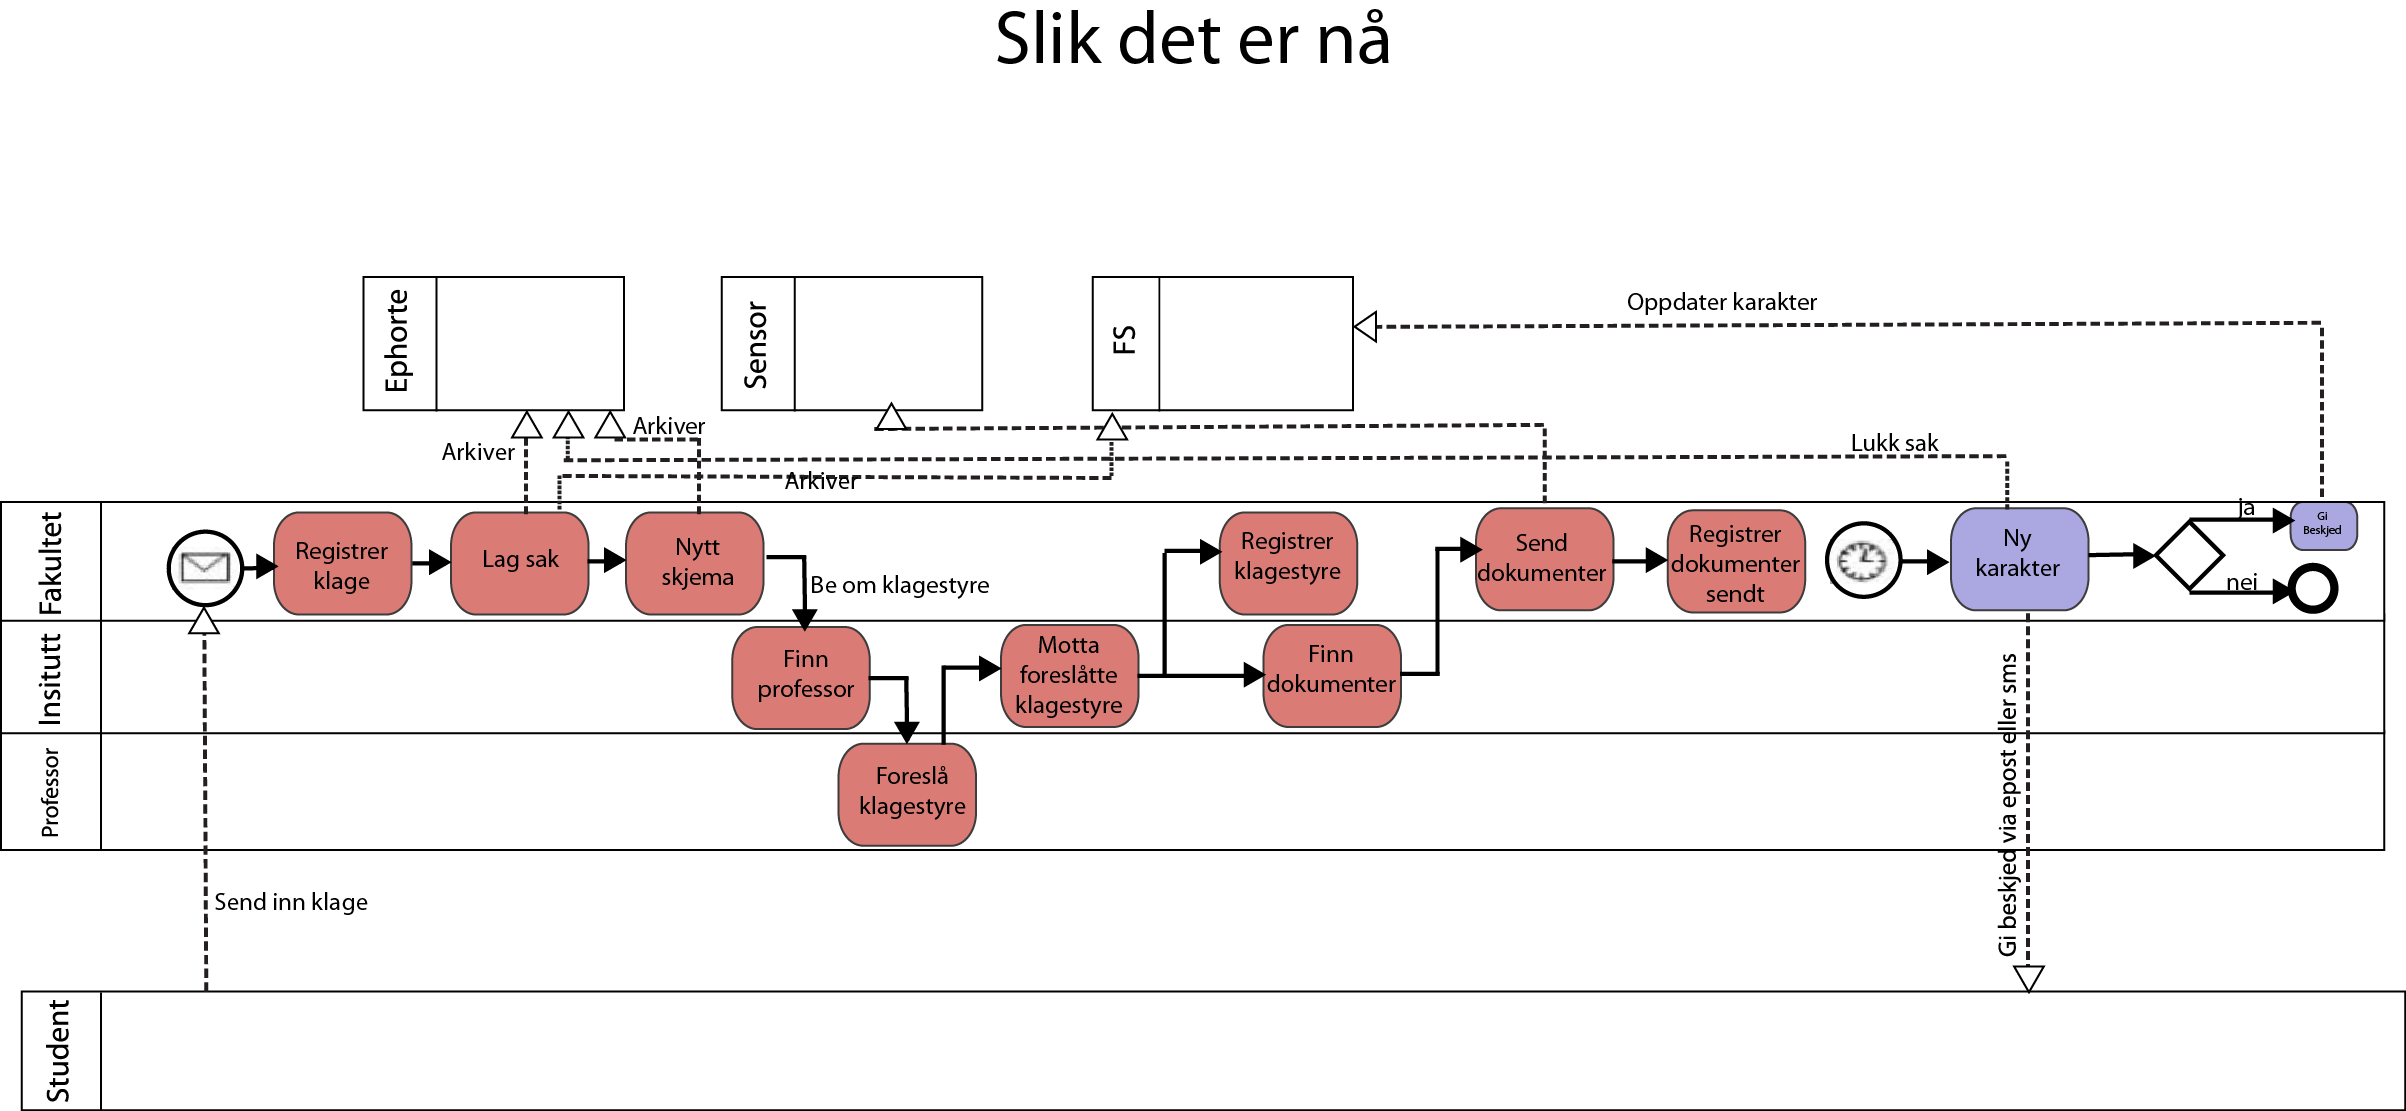
\includegraphics[width=0.9 \textwidth]{before.png}

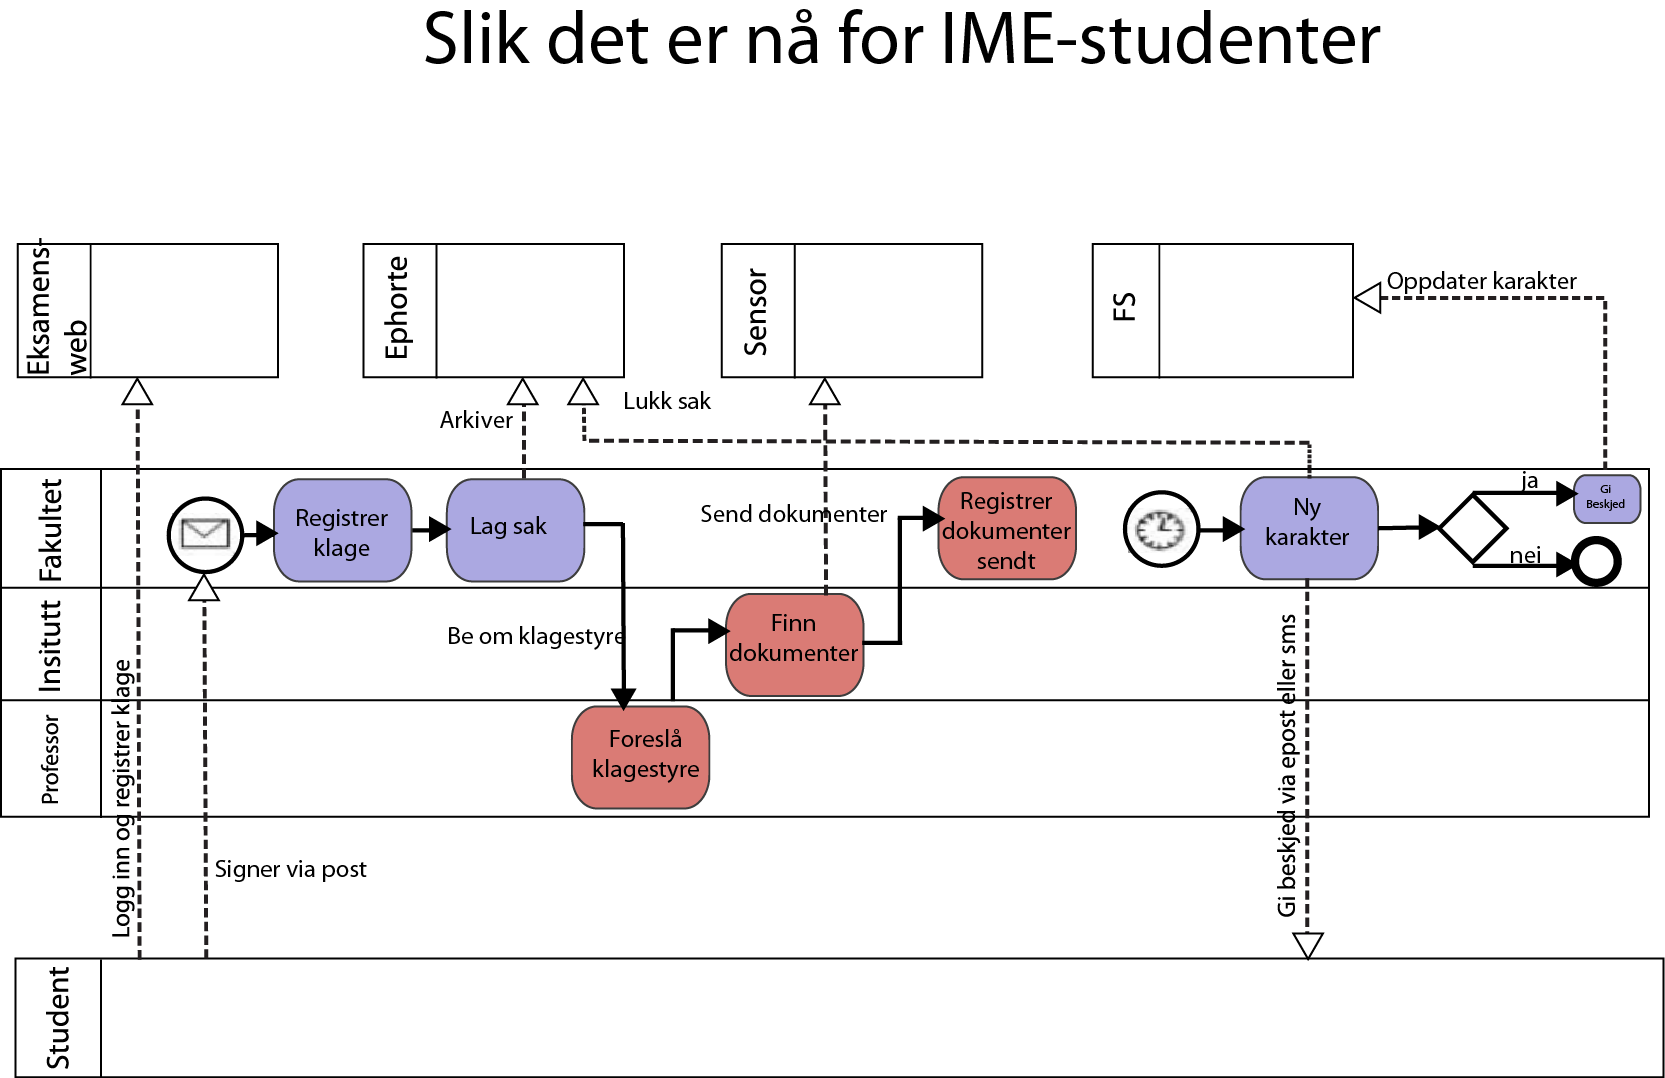
\includegraphics[width=0.9 \textwidth]{eksamensweb_ny.png}

\section{Slik systemet er idag}
Situasjonen i dag er at Studentweb, Eksamensweb og itslearning er tre separate løsninger.  Den eneste interaksjonen som finnes mellom løsningene er at Its Learning henter informasjon om hvilke fag en student er undervisningsmeldt til fra FS. FS er datagrunnlaget til Studentweb. De tre løsningene benytter alle av Feide, noe som gjør at dersom du logger inn på en av løsningene, er de innlogget på de to andre i tillegg. 

\subsection{Studentweb}

Studentweb er studentenes grensesnitt for å administrere sine studier. Studentweb gjør det mulig for studenter å melde seg opp til fag på NTNU, registrere adresse, sjekke karakterer, bestille karakterutskrift, registrere ved hvilke fakultet de ønsker å stemme og få betalingsinformasjon om semesteravgift. Studentweb er utviklet i samarbeid med NTNU og de andre universitetene og høyskolene som benytter seg av systemet, og henter informasjon fra FS. 

\subsection{Itslearning}

Itslearning er blant verdens ledende opplæringsplattformer som er utviklet spesielt for utdanningssektoren. Plattformen støtter både lærere og studenter gjennom hele læringsprosessen. \url{http://www.itslearning.no/produkt}. Itslearning er en hyllevare NTNU benytter seg av, og fungerer som en kommunikasjonsarena mellom studenter og ansatte. De innebygde funksjonene i itslearning er mange; studenter kan for eksempel  lage studentgrupper, profesorer kan legge ut informasjon om øvingsopplegg og fag, og studenter har mulighet til å levere og få tilbakemeldinger på arbeid.

\subsection{Eksamensweb}
Eksamensweb er et webbasert klagesystem utviklet av og for IME-fakultetet på NTNU. Studenter som tar fag som er underlagt instituttene på IME-fakultetet kan registrere klage- og begrunnelsessaker på nettet. Studenter må allikevel signere skriftlig på både klage- og begrunnelsessaker. Selve prosessen med å behandle klage- og begrunnelsessaker forenkles ikke spesielt for faglærerne og sensorene, men ved å bruke eksamensweb har faglærerne en komplett oversikt over hvilke saker som venter på behandling. I arkivet finnes det i tillegg en komplett oversikt over tidligere behandlede saker. Faglærerne får i tillegg purringer fra systemet om saker som ikke har blitt behandlet. Dette fører til at saker ikke uforvarende blir glemt. Slik systemet fungerer i dag har man ikke mulighet til å be om begrunnelse eller klager på emner som ikke tilhører IME.
\url{https://secure.ime.ntnu.no/utvikling/aktiv/klagesaker/bruksanvisning.html}


\section{Forslag til endringer}
Vi ønsker å digitalisere begrunnelse- og klageprosessen på NTNU. Eksamensweb er en start på en elektronisk klageprosess, men denne er ikke optimal.

\subsection*{Eksamensweb og Studentweb}
I vårt nye system vil eksamensweb fungere som en plugin til studentweb. I dette nye systemet vil man ha de samme mulighetene som studentweb har i dag, men i tillegg vil studenten kunne be om begrunnelse og klage direkte i systemet, noe som gjør det mer oversiktlig. Denne løsningen vil optimalt kutte ledd i klageprosessen. Ved å gjøre alt elektronisk blir det mindre jobb for NTNU å motta begrunnelser/klager og for studentene å be om begrunnelse / klage.

Informasjonen som ligger på Studentweb i dag regnes ikke som sensitiv, og innlogging via Feide regnes derfor som sikker nok. Erik Langbakk som er ansvarlig for klager på fakultetet IME, forteller at klage- og begrunnelsesprosessen på NTNU krever signatur. For å unngå å måtte levere et skjema med underskrift manuelt, ønsker vi å benytte oss av en løsning i likhet med den Lånekassen bruker. Her signerer man med noe som heter Buypass. Buypass er registrert hos Post- og teletilsynet som utsteder av kvalifisert ID i henhold til lov om elektronisk signatur \url{http://www.buypass.no/om-buypass}. Vi ønsker fremdeles at muligheten for å signere manuelt forblir, slik at det ikke blir et krav om å skaffe seg buypass.


\subsection*{ItsLearning}
Etter et intervju med Jan Sverre Rønning som jobber med Its learning på NTNU fikk vi forklart at Its Learning og Studentweb tilbyr to forskjellige tjenester som det ikke ville vært lønnsomt for hverken studenter eller ansatte å slå de sammen. Han sa videre at It’slearning er en hyllevare, dette vi si at NTNU ikke kan gjøre noen endringer i dette systemet. For å gjøre endringer må det lages noe nytt, noe som vil føre til store kostnader.


\subsection{Nye StudentWeb}

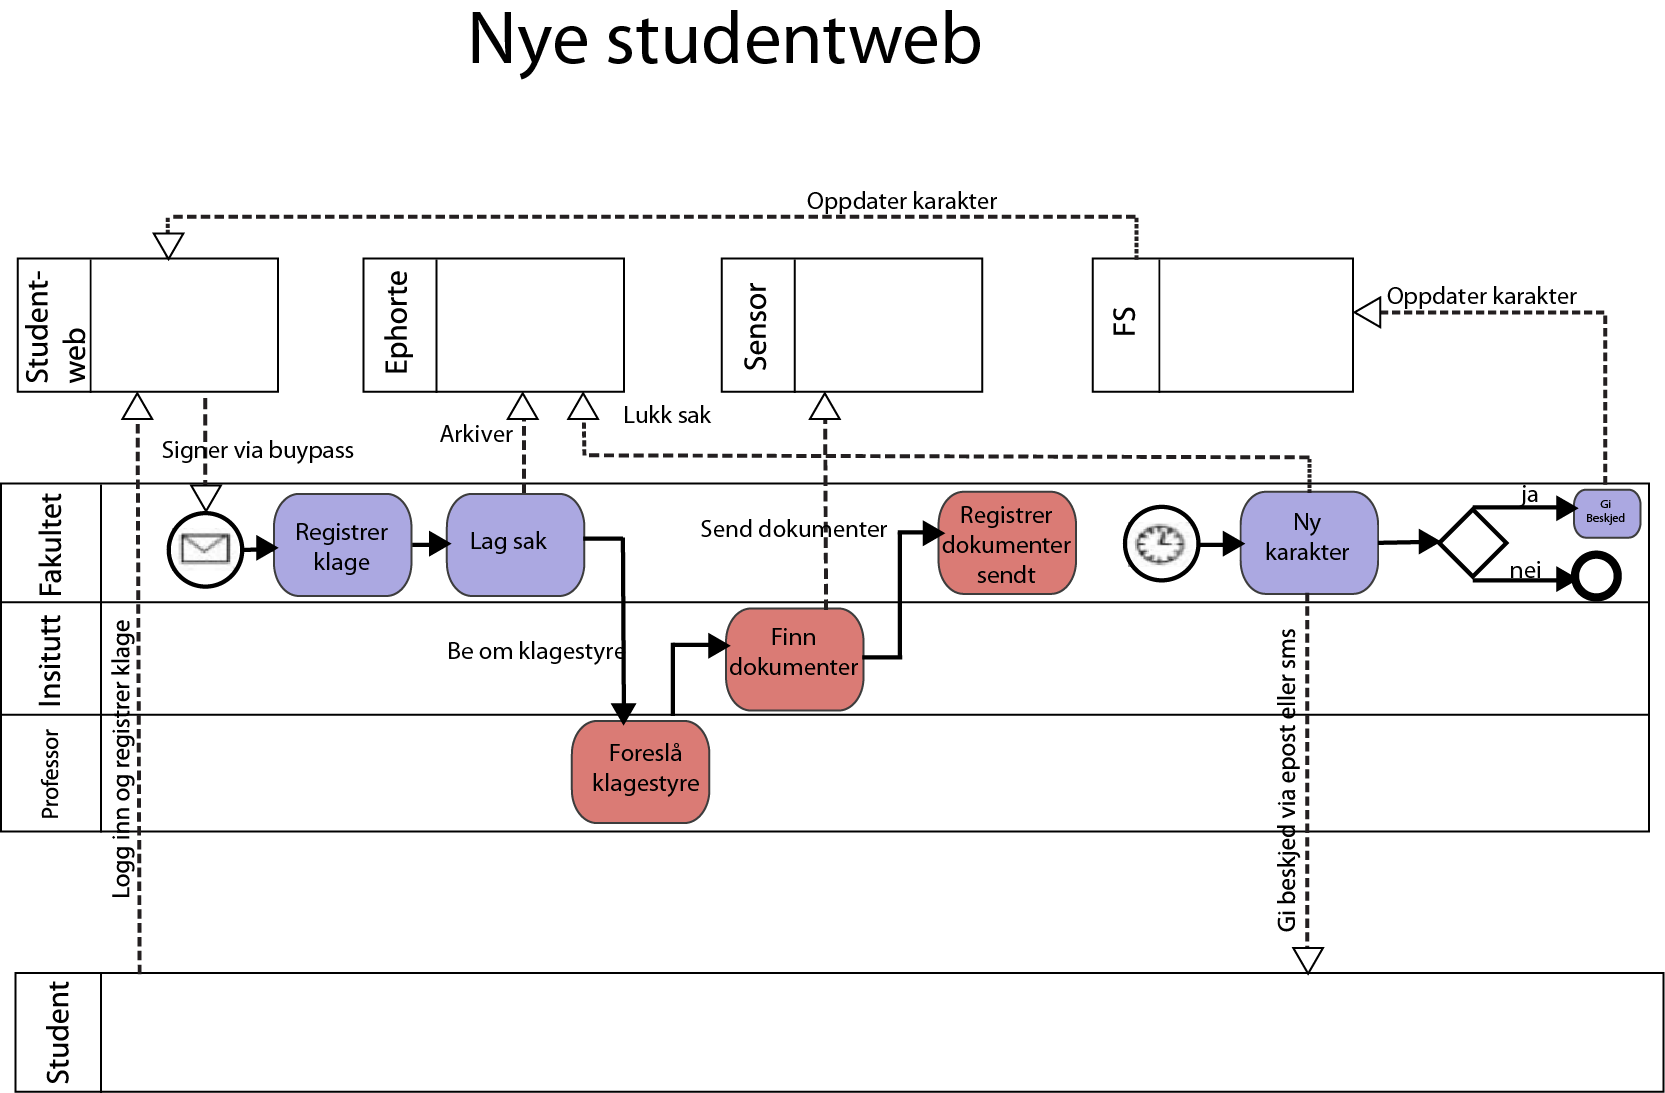
\includegraphics[width=0.9 \textwidth]{nyestudentweb}

\subsubsection*{Happy path:}

Student registrerer klage og får ny karakter på studentweb

\subsubsection*{Exception path:}

\begin{itemize}
\item Ingen internett tilgang
\item Studenten signerer ikke
\item Studentene har ikke innlogginsrett
\end{itemize}

\subsubsection*{Tekstlig beskrivelse:}

\begin{itemize}
\item Studenten registrerer klage og signerer via buypass eller skriftlig dokumentasjon
\item Fakultetet mottar klage, lager ny sak og ber om klagestyre
\item Professor foreslå klagestyre
\item Institutt finner dokumenter og sender disse til sensor
\item Fakultetet registrerer at dokumenter er sendt
\item Sensor setter karakter
\item Fakultetet registrerer karakter, og sender beskjed til studenten via sms eller epost
\begin{enumerate}
\item Karakteren er uendret - saken er ferdig
\item Karakteren er ny - oppdateres i FS og blir synlig i studentweb
\end{enumerate}
\end{itemize}

\section{Krav}

\subsection{Oppgavetabeller}

\subsubsection*{Oppgave 1: Innlogging på studentWeb}

\underline{Formål:} Oppnå personling og sikker tilgang til studentWeb\\
\underline{Hyppighet:} 100/time\\
\underline{Kritisk:} August og Januar

\begin{tabularx}{\textwidth}{|l|X|}
  \hline
  Underoppgave & Løsning \\ \hline
  Tilby en alternativ innlogging & Implementere Buypass som alternativ innlogging til studentWeb \\ \hline
\end{tabularx}

\subsubsection*{Oppgave 2: Registrere klage}

\underline{Formål:} Registrere klage i systemet\\
\underline{Hyppighet:} 4/time i kritisk periode\\
\underline{Kritisk:} August og Januar

\begin{tabularx}{\textwidth}{|l|X|}
  \hline
  Underoppgave & Løsning \\ \hline
  Verifiser student/fagkombinasjon & Sjekk om student er registret i faget \\ \hline
  Sikker innlogging & Innlogging med BuyPass \\ \hline
\end{tabularx}


\subsubsection*{Oppgave 3: Ny sak}

\underline{Formål:} Opprette ny klagesak\\
\underline{Hyppighet:} 4/time i kritisk periode\\
\underline{Kritisk:} August og Januar

\begin{tabularx}{\textwidth}{|l|X|}
  \hline
  Underoppgave & Løsning \\ \hline
  Lagre saken & Arkiver sak hos Ephorte \\ \hline
  Opprette klage & Gi beskjed til professor om å opprette et klagestyre \\ \hline
  Tilgang til dokumenter & Be instituttet sende relevante papirer til sensor \\ \hline
\end{tabularx}

\subsubsection*{Oppgave 4: Ny karakter}

\underline{Formål:} Oppdatere karakter etter klage\\
\underline{Hyppighet:} Sjeldent\\
\underline{Kritisk:} Menneskelig svikt (skrivefeil og lignende)

\begin{tabularx}{\textwidth}{|l|X|}
  \hline
  Underoppgave & Løsning \\ \hline
  Beskjed til student & Send epost til student \\ \hline
  Endre karakter & Send ny karakter til FS og videre til StudentWeb. \\ \hline
  Avslutte sak & Send beskjed til Ephorte for å avslutte saken \\ \hline
\end{tabularx}

\subsection{Funksjonelle krav}

Under er det listet noen funksjonelle krav for forslag til det nye systemet. Disse kravene omhandler mye sikkerhet da dette er veldig viktig i forhold til den nye
implementasjonen av systemet. 

\begin{tabularx}{\textwidth}{|l|X|}
  \hline
  \underline{Navn} & FK1 \\ \hline
  \underline{Viktighet} & Høy \\ \hline
  \underline{Formål} & Innsending av klage fra StudentWeb \\ \hline
  \underline{Krav} & StudentWeb skal tilby digital innsending av klage på karakter \\ \hline
  \underline{Tiltak} & Implementere en modul til StudentWeb som støtter digital klageinnsending \\ \hline
\end{tabularx}

\vfill

\begin{tabularx}{\textwidth}{|l|X|}
  \hline
  \underline{Navn} & FK2 \\ \hline
  \underline{Viktighet} & Medium \\ \hline
  \underline{Formål} & Driftsanalyse \\ \hline
  \underline{Krav} & Modulen skal rapportere alle feil til systemeier. \\ \hline
  \underline{Tiltak} & Unntakshåndteringen skal implementere e-postvarsling ved feil til systemeier. \\ \hline
\end{tabularx}

\vfill

\begin{tabularx}{\textwidth}{|l|X|}
  \hline
  \underline{Navn} & FK3 \\ \hline
  \underline{Viktighet} & Høy \\ \hline
  \underline{Trussel} & Identifisering \\ \hline
  \underline{Krav} & En gyldig norsk signatur er nødvendig for å sende inn klage \\ \hline
  \underline{Tiltak} & Implementere BuyPass som signaturform \\ \hline
\end{tabularx}

\vfill

\begin{tabularx}{\textwidth}{|l|X|}
  \hline
  \underline{Navn} & FK4 \\ \hline
  \underline{Viktighet} & Høy \\ \hline
  \underline{Trussel} & Autentisering \\ \hline
  \underline{Krav} & Løsningen skal ikke tilby digital innsending av klage med mindre buypass signeringen er validert \\ \hline
  \underline{Tiltak} & Validere autentifisering fra StudentWeb \\ \hline
\end{tabularx}

\vfill

\begin{tabularx}{\textwidth}{|l|X|}
  \hline
  \underline{Navn} & FK5 \\ \hline
  \underline{Viktighet} & Høy \\ \hline
  \underline{Trussel} & Immunitetskrav \\ \hline
  \underline{Krav} & Alle filer som blir lastet ned må skannes for malware. \\ \hline
  \underline{Tiltak} & Ha oppdatert anti-malware programvare til en hver tid \\ \hline
\end{tabularx}

\subsection{Ikke-funksjonelle krav}

\begin{tabularx}{\textwidth}{|l|X|}
  \hline
  \underline{Navn} & IFK1 \\ \hline
  \underline{Viktighet} & Høy \\ \hline
  \underline{Trussel} & Generell \\ \hline
  \underline{Krav} & Løsningen skal ikke undermine eksisterende sikkerhetsmekanismer i StudentWeb eller FS \\ \hline
  \underline{Tiltak} & Det skal ikke implementeres mekanismer som åpner for større tilgangsnivå av informasjon enn før implementasjon \\ \hline
\end{tabularx}

\vfill

\begin{tabularx}{\textwidth}{|l|X|}
  \hline
  \underline{Navn} & IFK2 \\ \hline
  \underline{Viktighet} & Høy \\ \hline
  \underline{Trussel} & Data Transport \\ \hline
  \underline{Krav} & Implementasjon må kreve sikker kommunikasjon med eksterne tilbydere \\ \hline
  \underline{Tiltak} & Implementere punkt-til-punkt kryptering mot systemene det integreres mot \\ \hline
\end{tabularx}

\vfill

\begin{tabularx}{\textwidth}{|l|X|}
  \hline
  \underline{Navn} & IFK3 \\ \hline
  \underline{Viktighet} & Medium \\ \hline
  \underline{Trussel} & Eksponering av indre mekanikker. \\ \hline
  \underline{Krav} & Hvis feil oppstår skal ikke feilbedskjeder avsløre systemet indre mekanikker for analyse. \\ \hline
  \underline{Tiltak} & Alle unntak og feil skal håndteres, "stacktrace" skjules for bruker og systemeier varsles. \\ \hline
\end{tabularx}

\vfill

\begin{tabularx}{\textwidth}{|l|X|}
  \hline
  \underline{Navn} & IFK4 \\ \hline
  \underline{Viktighet} & Høy \\ \hline
  \underline{Trussel} & Dataintegritet \\ \hline
  \underline{Krav} & Implementasjonen skal ikke kunne korrumpere informasjon i datagrunnlaget (FS) \\ \hline
  \underline{Tiltak} & Klageinnsendingsmodulen vil ha begrenset lesetilgang til relevante posteringer i datagrunnlaget og skrivetilgang bare hvor relevant. \\ \hline
\end{tabularx}

\vfill

\begin{tabularx}{\textwidth}{|l|X|}
  \hline
  \underline{Navn} & IFK5 \\ \hline
  \underline{Viktighet} & Høy \\ \hline
  \underline{Trussel} & Innbrudd \\ \hline
  \underline{Krav} & Implementasjonen skal kunne detektere at den er under angrep. \\ \hline
  \underline{Tiltak} & Det skal implementeres monitorering der modulen vil kunne resonnere at den er under systematisk angrep, blir testet for sårbarheter eller at en funksjon er
  eksponert uten at forhåndskrav som f.eks.\ autentifisering er gjennomført av bruker. \\ \hline
\end{tabularx}

\vfill

\begin{tabularx}{\textwidth}{|l|X|}
  \hline
  \underline{Navn} & IFK5 \\ \hline
  \underline{Viktighet} & Høy \\ \hline
  \underline{Trussel} & Personvern \\ \hline
  \underline{Krav} & Implementasjonen skal ikke gjøre synlig for andre brukere enn saksbehandlere eller klager hvem som har klag på fag. \\ \hline
  \underline{Tiltak} & Datagrunnlaget skal kreve at innsyn krever at brukeren som krever innsyn enten er den som har lagt inn klage eller saksbehandler tildelt relevant sak. \\ \hline
\end{tabularx}

\vfill

\begin{tabularx}{\textwidth}{|l|X|}
  \hline
  \underline{Navn} & IFK6 \\ \hline
  \underline{Viktighet} & Medium \\ \hline
  \underline{Trussel} & Overlevelse \\ \hline
  \underline{Krav} & Systemet skal være robust \\ \hline
  \underline{Tiltak} & Systemet skal kunne gi relevante feilbedskjeder dersom avhengighetssysterm som BuyPass eller datagrunnlaget er midlertidig utilgjengelig \\ \hline 
\end{tabularx}



\newpage
\subsection{Risikoanalyse}

\begin{tabular}{c l l}
    1. & Hendelse (H)\\
    2. & Sansynlighet (1-9) (S) \\
    3. & Innvirkning (1-9) (I) \\
    4. & Viktighet (V = S*I) \\
    5. & Preventative tiltak (P) \\
    6. & Reaktive tiltak (R) \\
\end{tabular}

\begin{tabular}{|p{0.2 \textwidth}|p{0.1 \textwidth}|p{0.1 \textwidth}|p{0.1 \textwidth}|p{0.2 \textwidth}|p{0.2 \textwidth}|} \hline
    H & S (1-9) & I (1-9) & V & P & R \\ \hline
    Person med nøkkeloppgave(r) i prosjektet blir borte over lengre tid & 5 & 8 & 40 & Ikke la personer få for stort ansvar & Redistribuering av ansvar \\ \hline
    Datatap & 3 & 6 & 18 & Backup, versjonskontroll og distribuering & Rulle tilbake til tidligere datagrunnlag \\ \hline
    Nedetid på servere & 9 & 6 & 54 & Redundans i form av flere servere og distribuert versjonskontroll & Kontakte teknisk personell \\ \hline
    Ugjevn arbeidsfordeling & 6 & 3 & 18 & Fordele oppgaver dynamisk & Redistribusjon av oppgaver \\ \hline
    For lite tid satt av til arbeidspakke & 7 & 5 & 35 & Bruke SCRUM og agile metoder & Redistribusjon av oppgaver \\ \hline
    Manglende støtte for kryptering i integrasjonssytemer & 3 & 7 & 21 & - & Implementere støttemoduler til integrasjonssystemet \\ \hline
    Gruppemedlemmer som ofte ikke møter på arbeidssesjoner & 9 & 1 & 9 & God kommunikasjon generelt og samkjøring av valg av kommunikasjonskanal & Disiplinering \\ \hline
    Risiko for at BuyPassløsningen er for krevende i bruk & 4 & 8 & 32 & Ha en backupløsning & Kontakte teknisk personell \\ \hline
    %TODO: Dukker ikke opp linje nederst
\end{tabular} 





\section{Drøfting av potensielle problemer man kan møte på i det nye systemet/ hva som kan være vanskelig}
	 	
En av de største svakhetene ved vårt forslag er at vi velger å ikke endre på Its Learning. Grunnen til dette er at Its Learning er et pakkeløsning som det er veldig vanskelig og dyrt å gjøre endringer på. Systemet i seg selv har mye bra funksjonalitet, men problemet ligger i at forelesere ikke bruker systemet. Dette har vi tenkt å adressere ved å synliggjøre Its Learning mer og ved å ha kursing i Its Learning for forelesere. Dette håper vi vil gjøre at flere forelesere tar i bruk systemet.

Et annet svakhet er at vi har lyst å bruke BuyPass til signering av klager på studentweb og dette innebærer at studentene må skaffe seg dette. Et stort risiko her er at studenter ikke skaffer seg BuyPass og dermed ikke tar i burk løsningen.

Løsningen vår innebærer at man får samlet både eksamensweb og studentweb på samme sted. Dette er et stort fordel
for brukere, men svakheten med denne løsningen er at man får et “single point of failure”, dvs.\ hvis studentweb går ned, er det heller ikke mulig å klage på eksamensresultater.

\section{Konklusjon}

\end{document}
